\documentclass[11pt]{article}
\usepackage[margin=0.9in]{geometry}
\usepackage{booktabs,multirow,array}
\usepackage{amsmath}
\usepackage{graphicx}
\usepackage[font=small,labelfont=bf]{caption}
\usepackage{enumitem}
\usepackage{xcolor}
\usepackage{hyperref}

\setlength{\parskip}{0.4em}
\setlength{\parindent}{0em}

\title{\Large\textbf{GAD+ Experiment Results}\\[4pt]
\normalsize Transition State Search with Eckart-Projected GAD and HIP}
\author{}
\date{April 2026}

\begin{document}
\maketitle
\thispagestyle{empty}

%----------------------------------------------------------------------
\section*{What This Is}

We benchmark \textbf{Gentlest Ascent Dynamics (GAD)} for finding transition states
using the HIP neural network potential on 300 organic reactions from Transition1x.
GAD modifies forces to ascend along the lowest Hessian eigenvector while descending
along all others:
$\mathbf{F}_{\text{GAD}} = \mathbf{F} + 2(\mathbf{F}\cdot\mathbf{v}_1)\mathbf{v}_1$.
A TS is converged when $n_{\text{neg}}=1$ (one negative eigenvalue in the
Eckart-projected vibrational Hessian) and force norm $< 0.01$ eV/\AA.
All methods are purely geometry-based---no path history. $\sim$25,000 total
optimizations across two rounds of experiments.

%----------------------------------------------------------------------
\section*{1. Noise Robustness \small(300 samples, dt=0.01, 300 steps)}

How does convergence degrade as we add Gaussian noise to the known TS geometry?

\begin{minipage}[t]{0.48\textwidth}
\centering
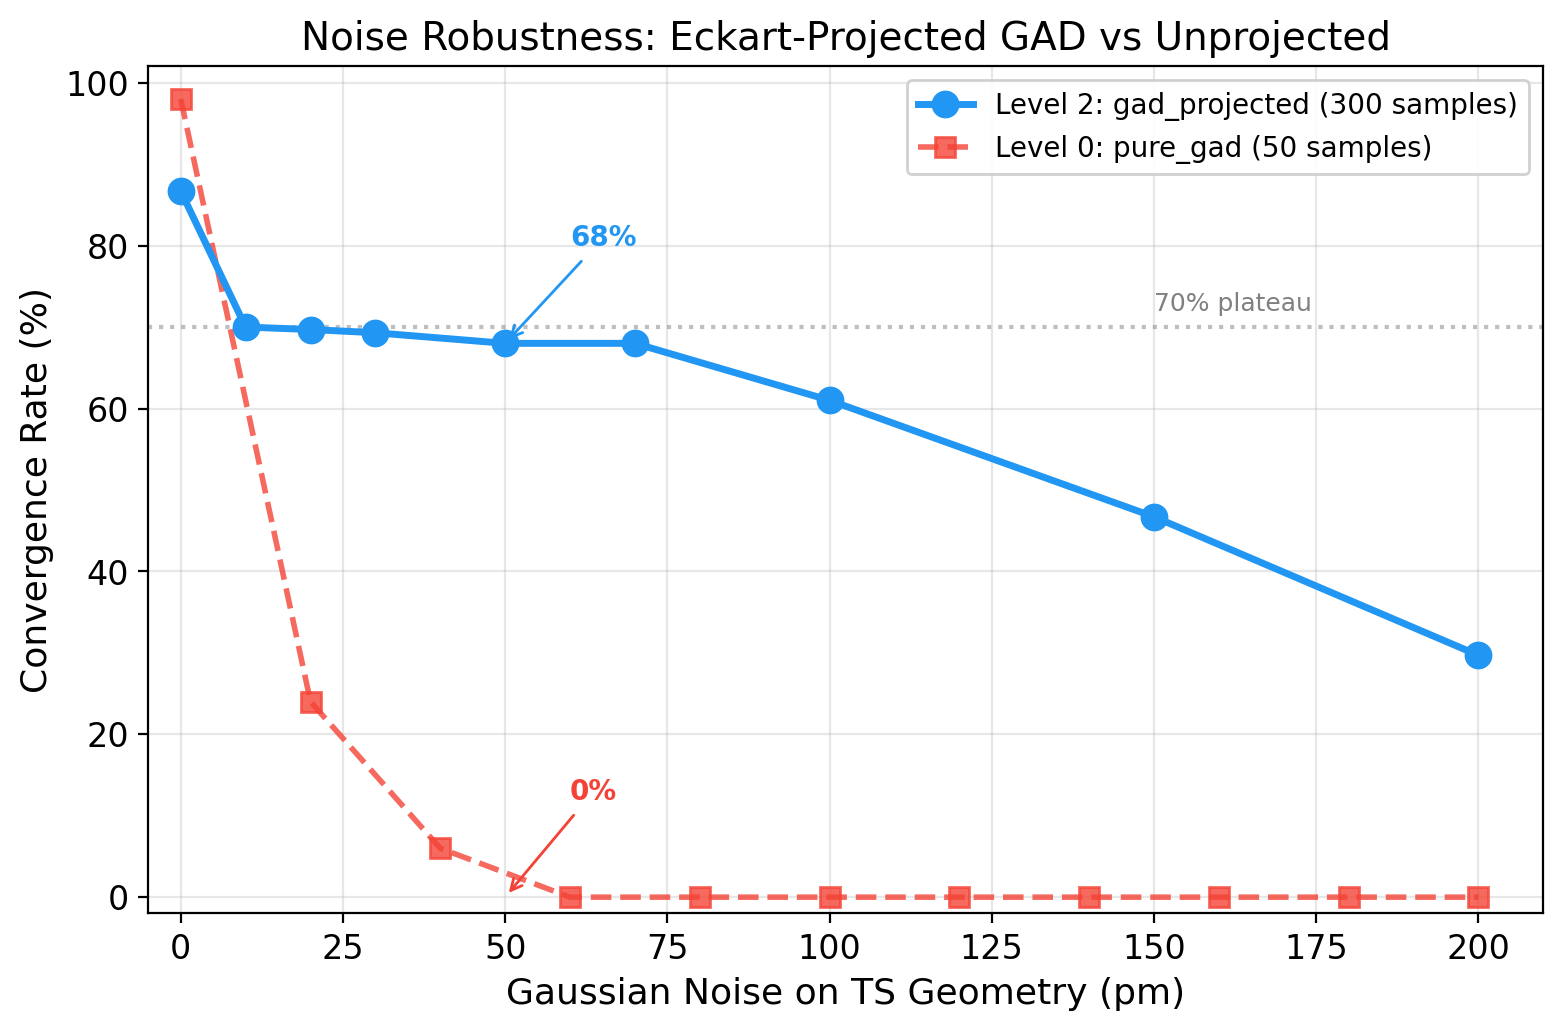
\includegraphics[width=\textwidth]{figures/fig1_conv_vs_noise.png}
\captionof{figure}{Level 2 (Eckart-projected, blue) vs Level 0 (unprojected, red).
Eckart projection is worth +68pp at 50pm.}
\end{minipage}\hfill
\begin{minipage}[t]{0.48\textwidth}
\centering
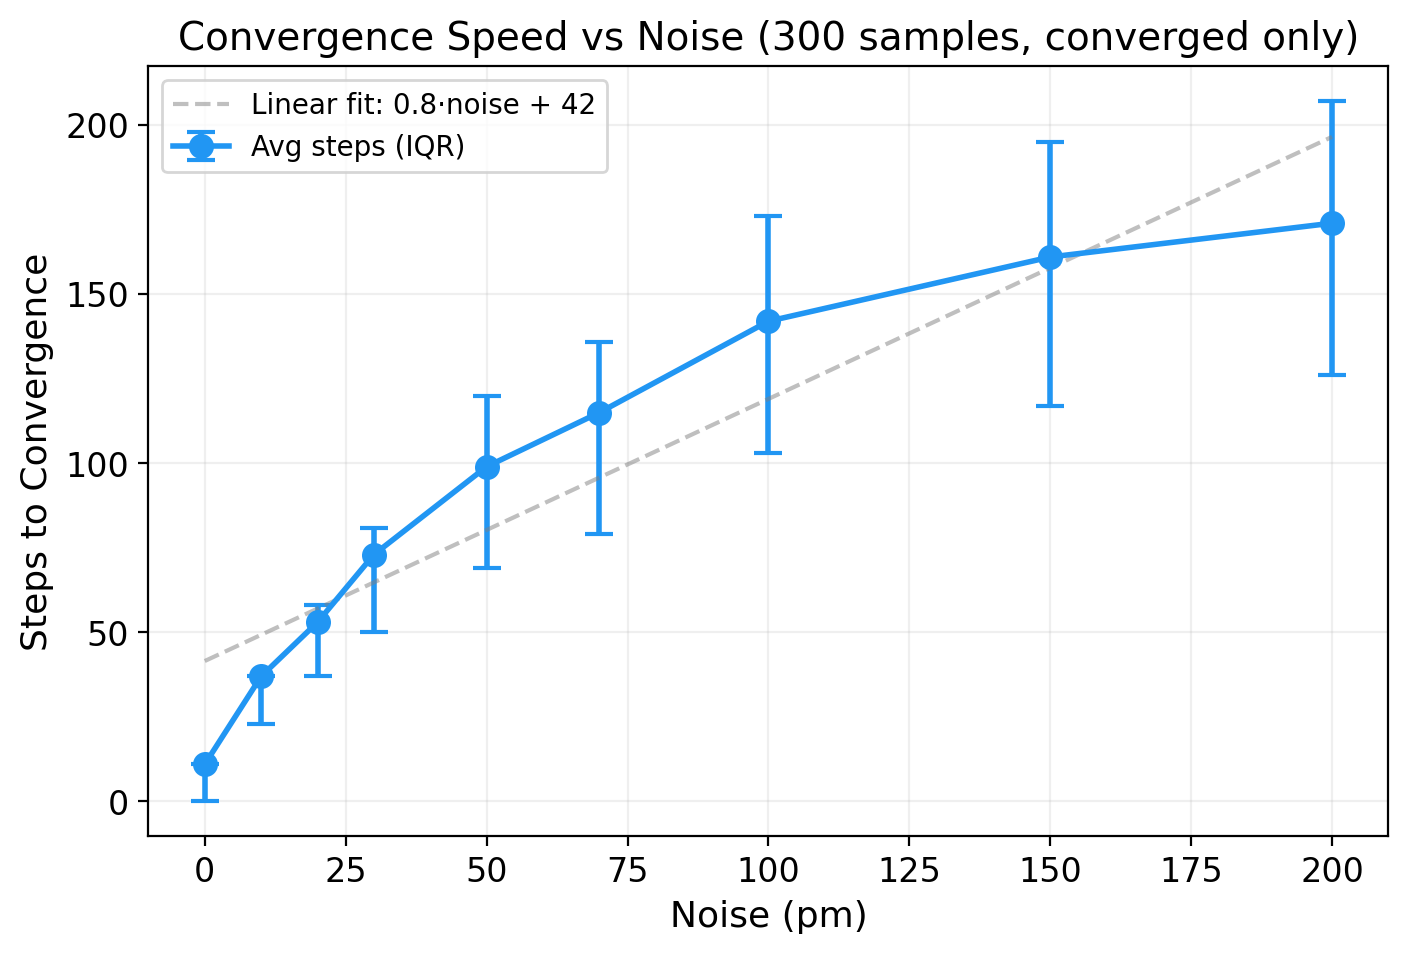
\includegraphics[width=\textwidth]{figures/fig6_steps_vs_noise.png}
\captionof{figure}{Steps to convergence scale linearly with noise.
Error bars show IQR.}
\end{minipage}

\vspace{0.5em}
\begin{tabular}{rrrr|rrrr}
\toprule
Noise & Conv & Rate & Steps & Noise & Conv & Rate & Steps \\
\midrule
0pm & 260/300 & 86.7\% & 11 & 70pm & 204/300 & 68.0\% & 115 \\
10pm & 210/300 & 70.0\% & 37 & 100pm & 183/300 & 61.0\% & 142 \\
20pm & 209/300 & 69.7\% & 53 & 150pm & 140/300 & 46.7\% & 161 \\
50pm & 204/300 & 68.0\% & 99 & 200pm & 89/300 & 29.7\% & 171 \\
\bottomrule
\end{tabular}

\textbf{Takeaway:} $\sim$70\% convergence plateau from 10--70pm. Level 0 (no projection)
gets 0\% at $\geq$50pm. Eckart projection is the single largest improvement.

%----------------------------------------------------------------------
\section*{2. Starting Geometry \small(300 samples, dt=0.01, 300 steps)}

Can GAD find a TS from geometries other than a noised TS?

\begin{minipage}[t]{0.48\textwidth}
\centering
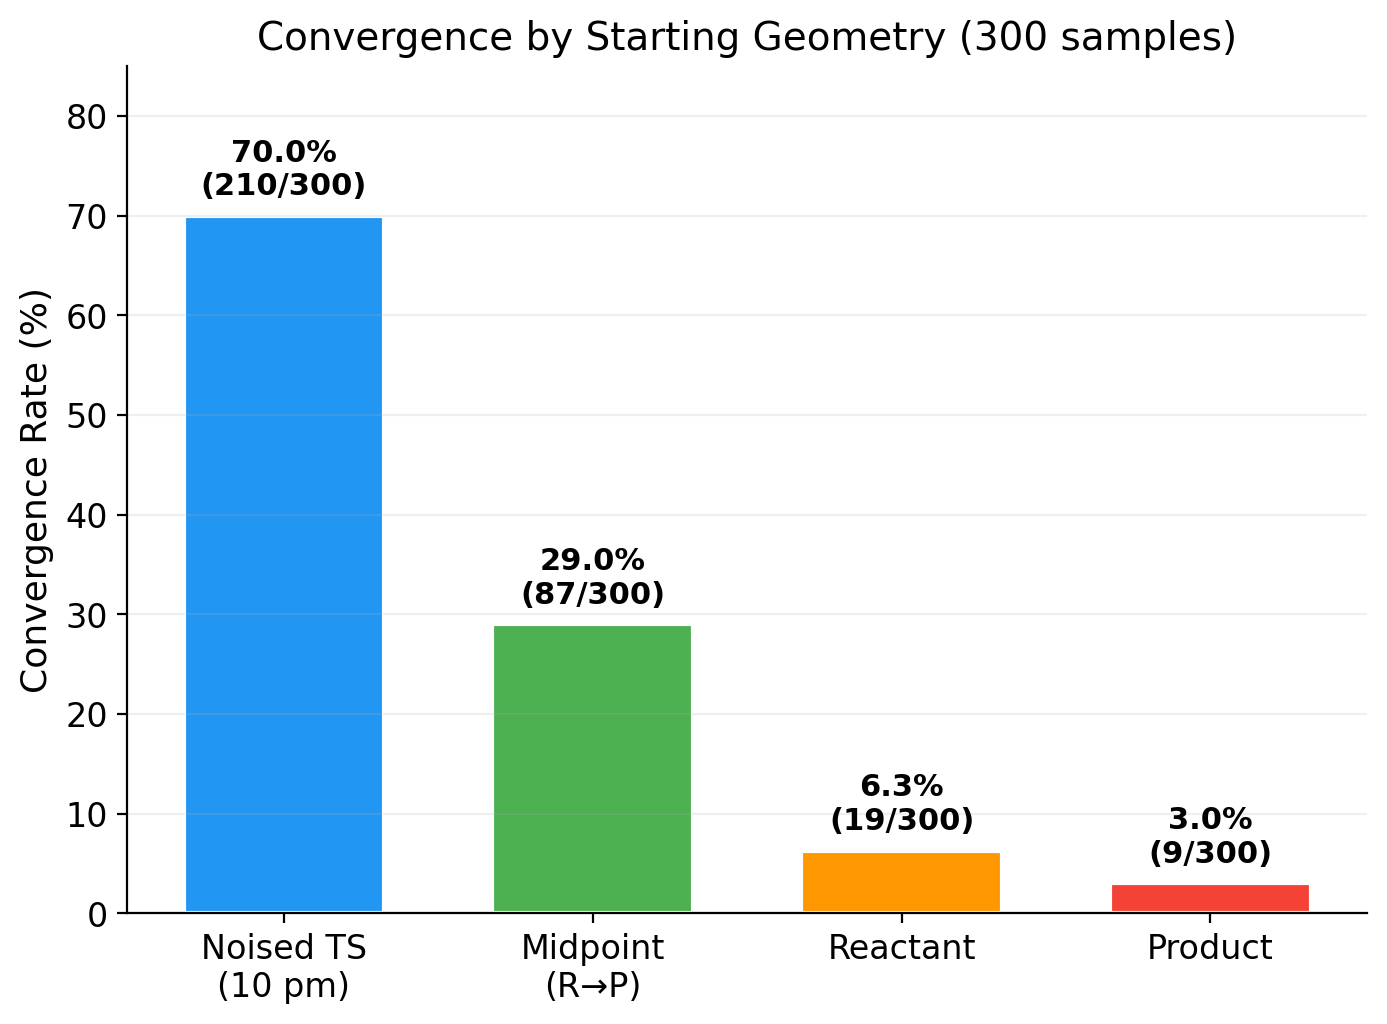
\includegraphics[width=\textwidth]{figures/fig2_starting_geometry.png}
\captionof{figure}{GAD needs saddle-region starts. Reactant/product
equilibria have $n_{\text{neg}}=0$, so GAD has no direction to ascend.}
\end{minipage}\hfill
\begin{minipage}[t]{0.48\textwidth}
\vspace{1em}
\begin{tabular}{lrrr}
\toprule
Start & Conv & Rate & Steps \\
\midrule
Noised TS & 210/300 & 70.0\% & 37 \\
Midpoint R$\to$P & 87/300 & 29.0\% & 191 \\
Reactant & 19/300 & 6.3\% & 108 \\
Product & 9/300 & 3.0\% & 65 \\
\bottomrule
\end{tabular}
\vspace{1em}

\textbf{Takeaway:} Midpoint interpolation is a viable
starting point (29\%) without knowing the TS.
Equilibrium geometries are near-useless.
\end{minipage}

%----------------------------------------------------------------------
\section*{3. Basin of Attraction \small(50 samples, dt=0.01, 300 steps)}

At what noise level does GAD start finding a \textit{different} TS?

\begin{minipage}[t]{0.55\textwidth}
\centering
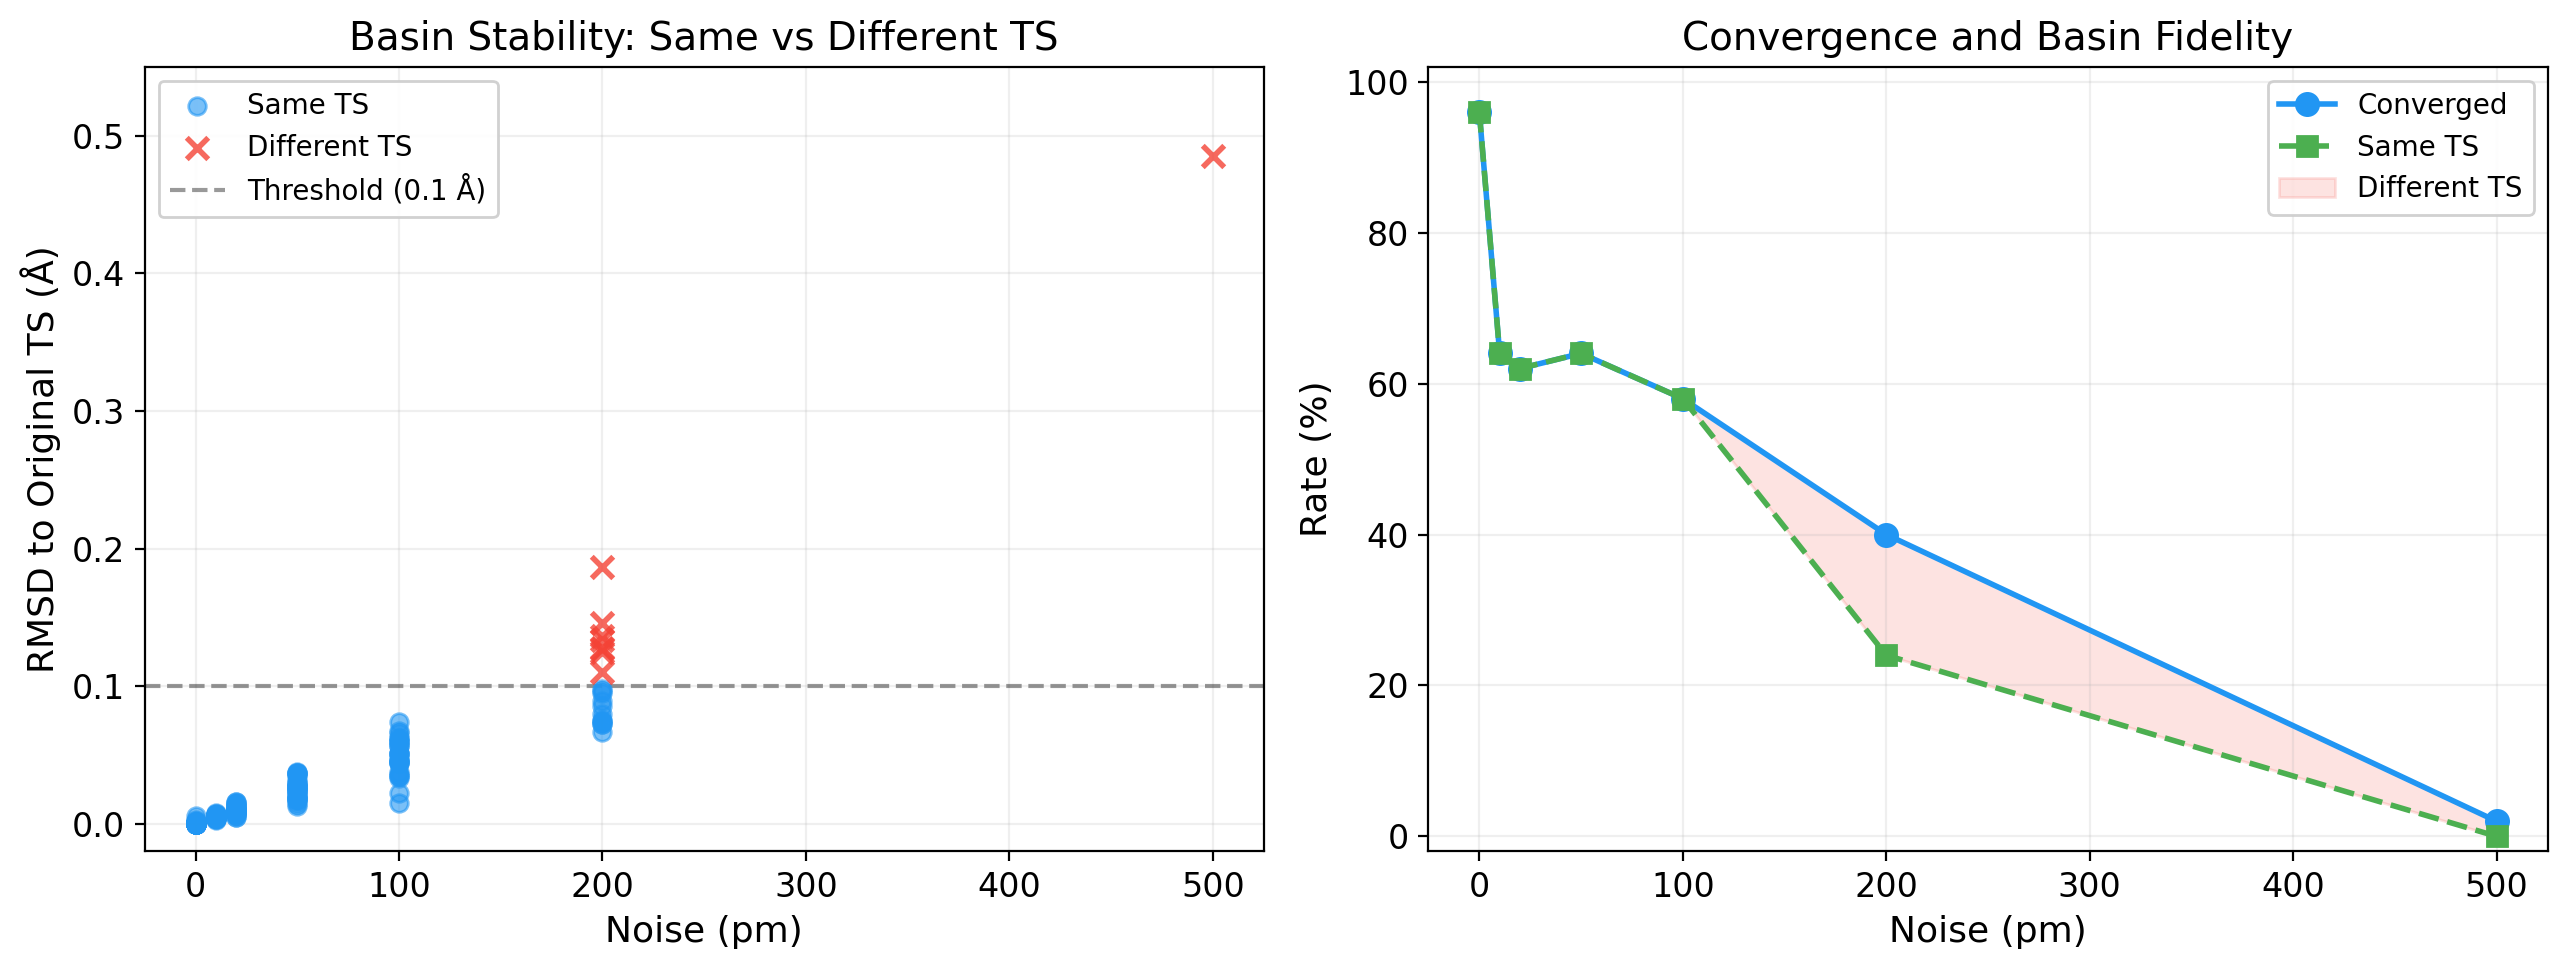
\includegraphics[width=\textwidth]{figures/fig3_basin_mapping.png}
\captionof{figure}{\textbf{Left:} RMSD to original TS (blue = same, red = different).
\textbf{Right:} Same-TS rate vs noise.}
\end{minipage}\hfill
\begin{minipage}[t]{0.40\textwidth}
\vspace{0.5em}
\begin{tabular}{rrrr}
\toprule
Noise & Conv & Same & Diff \\
\midrule
0pm & 48/50 & 48 & 0 \\
10pm & 32/50 & 32 & 0 \\
50pm & 32/50 & 32 & 0 \\
100pm & 29/50 & 29 & 0 \\
200pm & 20/50 & 12 & 8 \\
500pm & 1/50 & 0 & 1 \\
\bottomrule
\end{tabular}
\vspace{0.5em}

\textbf{Takeaway:} Basin stable to 100pm---\textbf{zero wrong TS found} in 172
converged runs. GAD is either right or fails. No silent errors.
\end{minipage}

%----------------------------------------------------------------------
\section*{4. Round 1: 7-Method Comparison \small(300 samples, 1000 steps)}

\begin{center}
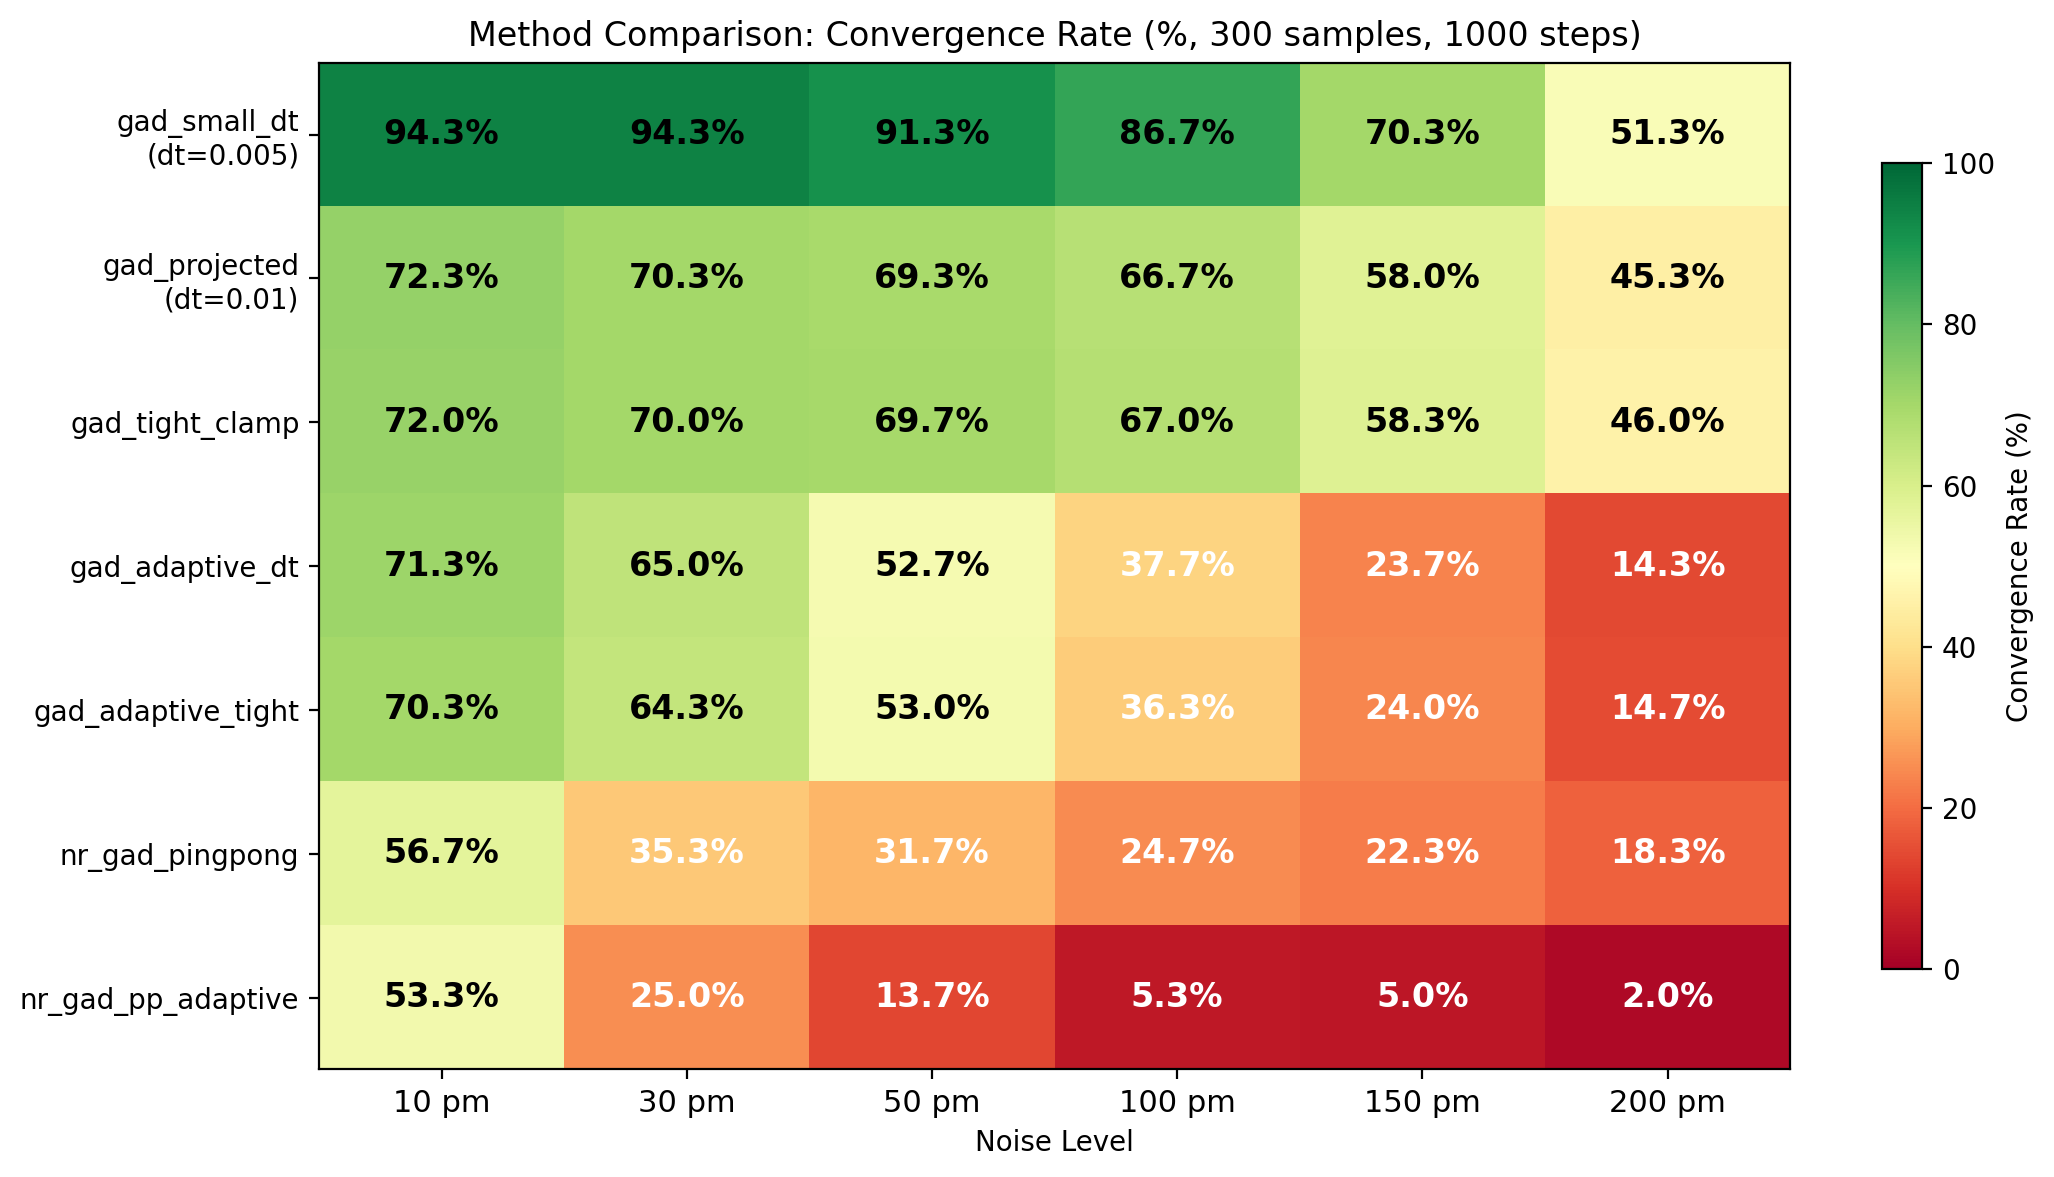
\includegraphics[width=0.85\textwidth]{figures/fig4_method_heatmap.png}
\captionof{figure}{Convergence rate heatmap. \texttt{gad\_small\_dt} (dt=0.005) dominates
everywhere. Adaptive dt and NR-GAD ping-pong both hurt.}
\end{center}

\begin{tabular}{l*{6}{r}}
\toprule
Method & 10pm & 30pm & 50pm & 100pm & 150pm & 200pm \\
\midrule
\textbf{gad\_small\_dt (dt=0.005)} & \textbf{94.3} & \textbf{94.3} & \textbf{91.3} & \textbf{86.7} & \textbf{70.3} & \textbf{51.3} \\
gad\_projected (dt=0.01)  & 72.3 & 70.3 & 69.3 & 66.7 & 58.0 & 45.3 \\
gad\_tight\_clamp         & 72.0 & 70.0 & 69.7 & 67.0 & 58.3 & 46.0 \\
gad\_adaptive\_dt         & 71.3 & 65.0 & 52.7 & 37.7 & 23.7 & 14.3 \\
nr\_gad\_pingpong         & 56.7 & 35.3 & 31.7 & 24.7 & 22.3 & 18.3 \\
nr\_gad\_pp\_adaptive     & 53.3 & 25.0 & 13.7 &  5.3 &  5.0 &  2.0 \\
\bottomrule
\end{tabular}

%----------------------------------------------------------------------
\section*{5. Round 2: Preconditioned GAD \small(300 samples, 1000 steps)}

\textbf{Idea:} $\Delta\mathbf{x} = dt \cdot |\mathbf{H}|^{-1} \mathbf{F}_{\text{GAD}}$. Scale each vibrational mode by $1/\max(|\lambda_i|, \text{floor})$---Newton-like step sizing. 30 MIG jobs, all 300/300 complete.

\begin{tabular}{l*{6}{r}}
\toprule
Method & 10pm & 30pm & 50pm & 100pm & 150pm & 200pm \\
\midrule
\textbf{gad\_small\_dt (baseline)} & \textbf{94.3} & \textbf{94.3} & \textbf{91.3} & \textbf{86.7} & \textbf{70.3} & \textbf{51.3} \\
precond\_gad\_001 (dt=0.005) & 73.7 & 61.0 & 48.0 & 21.7 & 7.3 & 3.3 \\
precond\_gad\_005            & 73.7 & 61.3 & 48.3 & 21.7 & 7.3 & 4.0 \\
precond\_gad\_01             & 72.7 & 62.7 & 47.0 & 21.0 & 7.3 & 4.3 \\
precond\_gad\_dt01 (dt=0.01) & 78.3 & 72.7 & 68.3 & 58.0 & 49.7 & 41.7 \\
\bottomrule
\end{tabular}

\textbf{Takeaway:} Preconditioning \textbf{hurts} GAD badly. At dt=0.005, $-21$pp at 10pm, $-43$pp at 50pm.
$|\mathbf{H}|^{-1}$ creates 100:1 step-size ratios between flat and steep modes,
starving the steep modes (often including the TS mode $\lambda_1$) of progress.
The eig\_floor (0.01--0.1) has no effect. Doubling dt to 0.01 partially recovers
but still underperforms plain GAD everywhere.

\textbf{Why:} Newton-like scaling helps descent toward \textit{minima}, but GAD navigates
a \textit{saddle} where all modes need uniform progress to maintain mode tracking.

%----------------------------------------------------------------------
\section*{6. Round 2: Smaller Timestep \& Adaptive dt \small(300 samples)}

\begin{tabular}{l*{6}{r}l}
\toprule
Method & 10pm & 30pm & 50pm & 100pm & 150pm & 200pm & Config \\
\midrule
\textbf{gad\_dt003} & \textbf{94.7} & \textbf{94.3} & \textbf{92.0} & \textbf{88.9} & \textbf{75.3} & \textbf{58.8} & dt=0.003, 2000 steps \\
gad\_small\_dt      & 94.3 & 94.3 & 91.3 & 86.7 & 70.3 & 51.3 & dt=0.005, 1000 steps \\
gad\_no\_clamp      & 94.3 & 94.3 & 91.3 & 86.7 & 70.9 & 54.6 & no disp cap \\
adaptive\_floor     & 83.0 & 80.0 & 70.2 & 43.2 & 26.5 & 15.9 & base=0.005, min=1e-3 \\
adaptive\_mm        & 53.7 & 40.2 & 35.1 & 22.6 & 12.4 & 5.7 & base=0.002 (MM-GAD) \\
adaptive\_mm2       & 40.1 & 29.6 & 22.4 & 13.1 & 6.3 & 2.4 & base=0.001 \\
\bottomrule
\end{tabular}

\textbf{Takeaways:}
\begin{itemize}[nosep,leftmargin=1.5em]
\item \textbf{dt=0.003 is the new best}: +2.2pp at 100pm, +5pp at 150pm, \textbf{+7.5pp at 200pm} vs dt=0.005.
      Smaller dt continues to help, especially at high noise.
\item \textbf{Displacement capping is inert}: gad\_no\_clamp $=$ gad\_small\_dt within noise.
\item \textbf{All adaptive dt variants fail.} Even corrected Multi-Mode GAD parameters (base=0.002): 54\% at 10pm.
      Eigenvalue-clamped adaptive dt is fundamentally incompatible with GAD dynamics.
\end{itemize}

%----------------------------------------------------------------------
\section*{7. Round 2: $\lambda_2$-Blended Preconditioned GAD \small(300 samples, 1000 steps)}

\textbf{Idea:} Smooth, differentiable alternative to hard n\_neg switching. Blend weight
$w = \sigma(k \cdot \lambda_2)$ controls whether to ascend $\mathbf{v}_1$:
\[
\mathbf{F}_{\text{blend}} = \mathbf{F} + 2w(\mathbf{F}\cdot\mathbf{v}_1)\mathbf{v}_1, \qquad
\Delta\mathbf{x} = dt \cdot |\mathbf{H}|^{-1} \mathbf{F}_{\text{blend}}
\]

\begin{tabular}{l*{6}{r}l}
\toprule
Method & 10pm & 30pm & 50pm & 100pm & 150pm & 200pm & Config \\
\midrule
precond\_descent    & 71.3 & 50.0 & 38.5 & 14.0 & 6.0 & 2.4 & hard switch, $w=0$ when $n_{\text{neg}}\geq 2$ \\
blend\_k50          & 72.0 & 50.0 & 37.2 & 14.3 & 6.2 & 3.1 & $\sigma(50\lambda_2)$ \\
blend\_k100         & 71.7 & 50.5 & 37.6 & 13.6 & 4.7 & 3.1 & $\sigma(100\lambda_2)$ \\
\bottomrule
\end{tabular}

\textbf{Takeaway:} All three are identical ($\sim$72\% at 10pm, $\sim$14\% at 100pm). The blend
weight $k$ doesn't matter---\textbf{the preconditioning dominates the failure mode.}
The $\sigma(k\lambda_2)$ mechanism is differentiable and correct, but it was tested on a
broken base ($|\mathbf{H}|^{-1}$ scaling). Re-test without preconditioning to isolate the
blend effect.

%----------------------------------------------------------------------
\section*{Summary}

\begin{center}
\begin{tabular}{rl}
\toprule
Finding & Evidence \\
\midrule
\textbf{Eckart projection is everything} & 0\% $\to$ 68\% at 50pm \\
\textbf{dt=0.003 is the new best} & 94.7\% at 10pm, 92\% at 50pm, 89\% at 100pm, 59\% at 200pm \\
\textbf{Basin stable to 100pm} & 0 wrong TS in 172 converged runs \\
\textbf{$|\mathbf{H}|^{-1}$ preconditioning hurts GAD} & $-$21pp at 10pm, $-$43pp at 50pm \\
\textbf{Adaptive dt always hurts} & 5 parameter sets tested, all worse than fixed dt \\
\textbf{NR switching hurts} & 4 variants (NR, damped NR, grad descent, precond) all worse \\
\textbf{Clamping: no effect} & No cap vs 0.05\AA\ cap, $<$1pp \\
\textbf{$\lambda_2$-blend needs re-test} & Mechanism correct, poisoned by preconditioning base \\
\bottomrule
\end{tabular}
\end{center}

\textbf{Best configuration:}
\texttt{gad\_dt003} --- Eckart-projected GAD, dt=0.003, 2000 steps, no mode tracking,
no adaptive dt, no preconditioning, no NR. \textit{The simplest method wins.}

\textbf{Next steps:}
\begin{enumerate}[nosep,leftmargin=1.5em]
\item $\lambda_2$-blended GAD \textit{without} preconditioning (isolate blend effect)
\item dt=0.002 and dt=0.001 with proportionally more steps
\item Multiple noise seeds for 95\% confidence intervals
\item Full Transition1x (9,561 samples)
\end{enumerate}

\end{document}
